\documentclass[a4paper, 12pt, oneside]{extarticle}
\input{$UNI/.templates/settings/preamble}
%shell-escape
\input{$UNI/.templates/settings/minted_settings.tex}
\usepackage{etoolbox} % пакунок для розширеного програмування
\usepackage{enumerate} % пакунок для розширеного програмування
\usepackage{amssymb}

\newtoggle{Report}
\togglefalse{Report}

\newtoggle{ShowVar}
\toggletrue{ShowVar} % якщо true, то відображається варіант замість теми
\renewcommand\Department{ОМП}

\newcommand\Type{\RGR}
\newcommand\Number{2}
\newcommand\Discipline{Теорія ймовірностей та математична статистика}
\newcommand\Topic{TOPIC}

\newcommand\Class{студент групи \Group}
\newcommand\Author{\Lname~\Initials}
\newcommand\Position{доцент}
\newcommand\Instructor{Білущак Г. І.}
\renewcommand\Variant{14}

\usepackage{pgfplots}
\pgfplotsset{compat=1.17}

\usepackage{boxedminipage}
\usepackage{varwidth}
\fboxrule=1pt

\usepackage{titlesec, blindtext, color}
\definecolor{gray75}{gray}{0.75}
\newcommand{\hsp}{\hspace{10pt}}
\titleformat{\chapter}[hang]{\Huge\bfseries}{\thechapter\hsp\textcolor{gray75}{|}\hsp}{0pt}{\Huge\bfseries}


\renewcommand{\thesubsection}{\arabic{subsection}}

\titleformat{\subsection}[hang]{\normalsize\bfseries}{\thesubsection{.}\hsp}{0pt}{\normalsize\normalfont}

% \usepackage{macrolist}
% \macronewlist{Answers}

% ЗАВДАННЯ
\newcommand{\Problem}{\subsection}
% РОЗВ'ЯЗОК
\newcommand{\Solution}{\subsubsection*{\centering \scshape Розв'язок:}}
% ВІДПОВІДЬ
\newcommand{\Answer}[1]{
\medskip
\null\hfill
\begin{boxedminipage}{\textwidth}
	\paragraph{Відповідь: }{#1}
	% \macrolistadd{Answers}{#1}
\end{boxedminipage}
}

\usetikzlibrary{patterns}

\begin{document}

\newgeometry{top=1cm,bottom=1cm,right=1.5cm,left=1.5cm}
\newcommand{\LINE}{\rule{\linewidth}{0.4mm}}
\begin{titlepage}
	\center

	\textsc{МІНІСТЕРСТВО ОСВІТИ І НАУКИ УКРАЇНИ}\\
	\textsc{НАЦІОНАЛЬНИЙ УНІВЕРСИТЕТ "`ЛЬВІВСЬКА ПОЛІТЕХНІКА"'}\\
	% \textsc{національний університет ``львівська політехніка''}\\
	\small
	\iftoggle{RGR} {}
	{
		{\Institute}\\
	}
	{кафедра \Department}\\
	[1.5cm]
	\normalsize
	%\large

	\includegraphics[scale=0.35]{$HOME/Templates/lpnu_doc_templates/lpnu_logo.png}\\[1.5cm]

	\iftoggle{Report}
	{
		\textsc{\LARGE\bfseries звіт}\\
		\textsc{ до \Type \, \No\Number}\\
	}
	{
		\textsc{\LARGE\bfseries \Type~\Number}\\
	}
до розрахунково-графічної роботи \\
  з дисципліни: "`\Discipline"'\\
  %на тему: \\

	\iftoggle{RGR}
	{
	\LINE\\[0.2cm] % норм?
	\large
		\textsc{\bfseries Варіант \Variant}\\[0cm]
	\LINE\\[1cm]
	}
	{
	\LINE\\[0.2cm]
	\large
	\textsc{\bfseries \Topic}\\[0cm]
	\normalsize
	\LINE\\[1cm]
	}


	\begin{flushright}
		\large
		\textit{Виконав}\\
		\normalsize
		\Class \; \textsc{\Author}

		\large
		\textit{Перевірив(ла)}\\
		\normalsize
		\Position \; \textsc{\Instructor}
	\end{flushright}

	\vfill
	Львів	\the\year{}
\end{titlepage}
\Margins


\setcounter{subsection}{2}

\Problem{
	а) Середня швидкiсть вiтру на данiй висотi дорiвнює 25 км/год. Оцiнити швидкiсть вiтру на
цiй висотi з ймовiрнiстю не меншою за 0.9, якщо $\sigma$ = 2.5 км/год.;
\\
	б) випадковi величини $\xi_1, \xi_2, ... , \xi_n, ...$ незалежнi i мають рiвномiрний розподiл $N(0; 1)$. Чи можна для цiєї послiдовностi застосовувати теорему Хiнчина ?
}

\paragraph{а)} За II нерівністю Чебишова:
% http://dspace.onu.edu.ua:8080/handle/123456789/12893
% http://matematika.martinmarinov.info/index.php?no=35
% https://ru.wikipedia.org/wiki/%D0%A2%D0%B5%D0%BE%D1%80%D0%B5%D0%BC%D0%B0_%D0%A5%D0%B8%D0%BD%D1%87%D0%B8%D0%BD%D0%B0_%E2%80%94_%D0%9A%D0%BE%D0%BB%D0%BC%D0%BE%D0%B3%D0%BE%D1%80%D0%BE%D0%B2%D0%B0
% https://uk.wikipedia.org/wiki/%D0%A2%D0%B5%D0%BE%D1%80%D0%B5%D0%BC%D0%B8_%D0%A5%D1%96%D0%BD%D1%87%D0%B8%D0%BD%D0%B0
$
{\displaystyle P\{|X-\eta |\geq \epsilon \}\leq {\frac {{\sigma }^{2}}{{\epsilon }^{2}}}}
\implies
0.9 \leq 6.25/\epsilon^2
\implies
0.9e^2 \leq 6.25
\implies
e^2 \leq 6.9(4)
\implies
e \leq 2.635231%38347364944324
$

% $
% P(\alpha < X < \beta) = \Phi(\frac{\beta - a}{\sigma}) - \Phi(\frac{\alpha - a}{\sigma})
% $.
% % Для нормального розподілу
% У нас симетричний інтервал, формула спрощується
% \begin{align}
% P(a-\delta < X < a + \delta) = \Phi \left( \frac{a + \delta - a}{\sigma} \right) - \Phi \left(\frac{a - \delta - a}{\sigma} \right)
% \\
% P(a-\delta < X < a + \delta) = \Phi \left( \frac{\delta}{\sigma} \right) - \Phi \left(\frac{-\delta}{\sigma} \right)
% =
% \Phi \left( \frac{\delta}{\sigma} \right) + \Phi \left(\frac{\delta}{\sigma} \right)
% = 2\Phi(\delta/\sigma)
% \end{align}

% $$
% % 0.9 = P \left\{ -\delta \leq \frac{\bar x_{\beta} - M(\xi)}{\sigma_{\xi/\sqrt{n}}} \leq \delta \right\}
% % \\
% 0.9 = 2\Phi(\delta/\sigma)
% \implies
% 0.45 = \Phi(\delta/2.5)
% \implies
% \delta/2.5 = 1.65
% \implies
% \delta = 4.125
% $$

\paragraph{б)}

$a = M_\xi = 0, \sigma^2 = 1, \epsilon \succ 0$

\begin{align}
\lim_{n\to\infty} P \left\{ \left| \frac{\sum \xi_n}{n}-a \right| \succ \epsilon \right\} = 0, \\
\lim_{n\to\infty} P \left\{ \left| \frac{\sum \xi_n}{n}-0 \right| \succ \epsilon \right\} = 0
\end{align}
% Коли стандартне відхилення 1, можемо вважати, що підмодульний вираз десь в околі 1 є, тому от.

\begin{minted}{r}
> bub <- function(x) { 1/sqrt(2*pi) * exp(-x^2/2) }
> bub(0.5)
[1] 0.3520653
> bub(21)
[1] 6.902029e-97
> bub(2)
[1] 0.05399097
> bub(3)
[1] 0.004431848
> bub(-3)
[1] 0.004431848
> bub(11)/11
[1] 1.926199e-28
> bub(100)/100
[1] 0
\end{minted}
Імовірність появи великих значень $\xi$ надзвичайно низька, тому можемо
вважати, що теорема виконується.

\Answer{
	% а) $ \xi \in [20.875; 29.125] $
	а) $ \xi \in [22.364769; 27.635231] $
	\-
	б) так.
}

\Problem{
	Дано розподiл двовимiрного дискретного випадкового вектора $(\xi, \eta)$:
	\\
	
\includegraphics[width=6cm]{4.png}
	\\
Знайти невiдому сталу a, розподiл компонент, коварiацiю. Перевiрити чи компоненти є
незалежними.
}

$$
0+0.05+0+0.1+.1+0.15+0.1+0.1+0+0.1+0.1+0.1=
.90
\implies a = 0.1
$$

\begin{minted}{r}
> xi <- c(-3, -3, -3, -3, -1, -1, -1, -1, 0, 0, 0, 0)
> eta <- c(-2, 0,   1,  5, -2,  0,  1,  5, -2, 0, 1,5)
> freq <- c(0, 0.05, 0, 0.1, 0.1, 0.15, 0.1, 0.1, 0.1, 0.1, 0.1, 0.1)
> distr <- data.frame(xi, eta, freq)
> distr
   xi eta freq
1  -3  -2 0.00
2  -3   0 0.05
3  -3   1 0.00
4  -3   5 0.10
5  -1  -2 0.10
6  -1   0 0.15
7  -1   1 0.10
8  -1   5 0.10
9   0  -2 0.10
10  0   0 0.10
11  0   1 0.10
12  0   5 0.10
\end{minted}

\subsubsection{Характеристики розподілу $\xi$}

\begin{minted}{r}
> xi_p <- c(sum(distr$freq[1:4]), sum(distr$freq[5:8]), sum(distr$freq[9:12]))
> xi_val <- c(-3, -1, 0)
> xi_dist <- data.frame(xi_val, xi_p)
> names(xi_dist) <- c('xi', 'p')
> xi_dist # розподіл величини ксі
  xi    p
1 -3 0.15
2 -1 0.45
3  0 0.40

> xi_dist$xi_p <- xi_dist$xi*xi_dist$p
> xi_dist$xi2_p <- xi_dist$xi*xi_dist$xi_p
> xi_dist
  xi    p  xi_p xi2_p
1 -3 0.15 -0.45  1.35
2 -1 0.45 -0.45  0.45
3  0 0.40  0.00  0.00

> m_xi <- sum(xi_dist$xi_p)
> m_xi
[1] -0.9
> m_xi2 <- sum(xi_dist$xi2_p)
> m_xi2
[1] 1.8
> d_xi <- m_xi2 - m_xi^2
> d_xi
[1] 0.99

> dev_xi = sqrt(d_xi)
> dev_xi
[1] 0.9949874
\end{minted}

\subsubsection{Те саме з $\eta$}

\begin{minted}{r}
> eta_val <- c(-2, 0, 1, 5)

# за допомогою ф-ї filter бібліотеки dplyr фільтруємо значення
> library(dplyr)
> eta_p <- c(sum((filter (distr, eta == -2))$freq), sum((filter(distr, eta == 0))$freq), sum((filter(distr, eta == 1))$freq), sum((filter(distr, eta == 5))$freq))
> eta_p
[1] 0.2 0.3 0.2 0.3

> eta_dist = data.frame(eta_val, eta_p)

> names(eta_dist) <- c('eta', 'p')

> eta_dist

  eta   p
1  -2 0.2
2   0 0.3
3   1 0.2
4   5 0.3

> eta_dist$eta_p <- eta_dist$eta*eta_dist$p
> eta_dist$eta2_p <- eta_dist$eta*eta_dist$eta_p

> eta_dist

  eta   p eta_p eta2_p
1  -2 0.2  -0.4    0.8
2   0 0.3   0.0    0.0
3   1 0.2   0.2    0.2
4   5 0.3   1.5    7.5

> m_eta = sum(eta_dist$eta_p)
> m_eta
[1] 1.3

> m_eta2 = sum(eta_dist$eta2_p)
> m_eta2
[1] 8.5

> d_eta = m_eta2 - m_eta^2
> d_eta
[1] 6.81

> dev_eta <- sqrt(d_eta)
> dev_eta
[1] 2.609598
\end{minted}

\subsubsection{Обчислення коваріації}
\begin{minted}{r}
> distr$xi_eta_p = distr$xi*distr$eta*distr$freq

> distr

   xi eta freq xi_eta_p
1  -3  -2 0.00      0.0
2  -3   0 0.05      0.0
3  -3   1 0.00      0.0
4  -3   5 0.10     -1.5
5  -1  -2 0.10      0.2
6  -1   0 0.15      0.0
7  -1   1 0.10     -0.1
8  -1   5 0.10     -0.5
9   0  -2 0.10      0.0
10  0   0 0.10      0.0
11  0   1 0.10      0.0
12  0   5 0.10      0.0
> sum(distr$xi_eta_p)

[1] -1.9
> m_xi_eta = sum(distr$xi_eta_p)

> cov_xi_eta = m_xi_eta - m_xi*m_eta
> cov_xi_eta
[1] -0.73
\end{minted}

\Answer{
	Коваріяція $= -0.73$
}

\Problem{
	Дано щiльнiсть неперервного випадкового вектора $(\xi, \eta)$:
	\\
	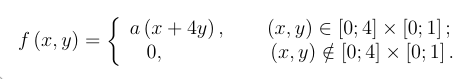
\includegraphics[width=9cm]{5.png}
	\\
	Знайти невiдому сталу a, розподiл компонент, коварiацiю.
}

% $$
% $$

\subsubsection{Пошук a}

\begin{minted}{r}
> library(pracma)
> integrand <- function(x, y) { x+4*y }
> integral2(integrand, 0, 4, 0, 1)
$Q
[1] 16

$error
[1] 8.881784e-16
\end{minted}

$$
16a = 1 \implies a = 1/16
$$

\subsubsection{Розподіл компонент}

$$
\frac{1}{16}\int_0^x dx \int_0^1 x+4y\, dy
% = \frac{1}{16}\int_0^x dx \left( xy + 4/2*y^2 \Big|_0^1 \right)
= \frac{1}{16}\int_0^x \left( x + 2 \right) \,dx
= \frac{1}{16} \left( x^2/2 + 2x \right) \Big|_0^x
= x^2/32 + x/8
$$

\begin{dmath}
\frac{1}{16}\int_0^4 dx \int_0^y x+4y\, dy
= \frac{1}{16}\int_0^4 dx \left( xy + 4/2*y^2 \Big|_0^y \right)
= \frac{1}{16}\int_0^4 dx \left( xy + 2y^2 \right)
= \frac{1}{16}\left( x^2y/2 + 2y^2x \Big|_0^4 \right)
= \frac{1}{16}\left( 8y + 8y^2 \right)
= 1/2*y + 1/2*y^2
\end{dmath}

\subsubsection{Коваріація}

$$
\text{cov}(x;y) = M_{xy} - M_xM_y %m_xi_eta - m_xi*m_eta
= (\ref{mxy}) - (\ref{mx})(\ref{my})
= 64/3 - 14/3 * 7/24 \approx 19.97222
$$

\fboxrule=0.5pt
\begin{boxedminipage}{\textwidth}
\begin{align}
	M_{xy} &= \int_0^4 \,dx \int_0^1 xy (x+4y) \,dy
		= \int_0^4 \frac{{x}^{2}}{2}+\frac{4\,x}{3} \,dx
		= \frac{{x}^{3}}{6}+\frac{2\,{x}^{2}}{3} \Bigg|_0^4
		= 64/3
		\label{mxy}
\\
	M_x &= \int_0^4 x(x^2/32 + x/8) \,dx = \frac{{x}^{4}}{128}+\frac{{x}^{3}}{24} \Bigg|_0^4 = 14/3
	\label{mx}
\\
	M_y &= \int_0^1 y(y/2 + y^2/2) \,dy = \frac{{y}^{4}}{8}+\frac{{y}^{3}}{6} \Bigg|_0^1 = \frac{7}{24}
	\label{my}
\end{align}
\end{boxedminipage}

\fboxrule=1pt

\Answer{
$a=1/16$.
Розподіл $x$: $x^2/32 + x/8$.
Розподіл $y$: $y/2 + y^2/2$.
$\text{cov}(x;y) = 19.97222$.
}

\Problem{
Ювiляру подарували 25 букетiв. Кiлькiсть квiтiв у них була такою: 3, 5, 5, 7, 5, 7, 5, 5,
3, 5, 5, 9, 7, 3, 3, 5, 5, 5, 7, 3, 5, 5, 3, 3, 5. Записати статистичний i варiацiйний ряд.
Знайти
розмах вибiрки,
моду,
медiану.
Обчислити
середнєзначення,
вибiркову i незмiщену
дисперсiї,
асиметрiю,
ексцес,
коефiцiєнт варiацiї,
емпiричну функцiю розподiлу
i полiгон частот.
}
% 3, 5, 5, 7, 5, 7, 5, 5, 3, 5, 5, 9, 7, 3, 3, 5, 5, 5, 7, 3, 5, 5, 3, 3, 5

% \begin{table}
% $$
% \begin{array}{cc}
% x_i & n_i \\
% 3 & 7 \\
% 5 & 13 \\
% 7 & 4 \\
% 9 & 1
% \end{array}
% $$
% 	\caption{варіаційний ряд}
% \end{table}
Підготуємо дані:
\begin{minted}{r}
> raw_6 <- c(3, 5, 5, 7, 5, 7, 5, 5, 3, 5, 5, 9, 7, 3, 3, 5, 5, 5, 7, 3, 5, 5, 3, 3, 5)
> x_i = c(3,5,7,9)
> n_i = c(7,13,4,1)
> var_6 <- data.frame(x_i, n_i) # варіаційний ряд
\end{minted}

\subsubsection{Розмах вибiрки, мода, медiана, дисперсії}

Розмах вибірки: $9-3 = 6$

\begin{minted}{r}
> var_6
  x_i n_i
1   3   7
2   5  13 # мода — 5
3   7   4
4   9   1
> summary(var_6)
      x_i           n_i
 Min.   :3.0   Min.   : 1.00
 1st Qu.:4.5   1st Qu.: 3.25
 Median :6.0   Median : 5.50 # медіана
 Mean   :6.0   Mean   : 6.25 # середнє значення
 3rd Qu.:7.5   3rd Qu.: 8.50
 Max.   :9.0   Max.   :13.00

> var(raw_6)  # вибіркова дисперсія
[1] 2.493333
\end{minted}

для отримання незміщеної оцінки генеральної дисперсії,
обчислимо скориговану дисперсію (домноживши вибіркову на $n$ і поділивши на $n-1$):

\begin{minted}{r}
> variance_6 = var(raw_6)*length(raw_6)/(length(raw_6)-1)
[1] 2.597222
\end{minted}

% \begin{minted}{r}
% > var_6$m_3 <- ((var_6$x_i - mean(raw_6))^3 * var_6$n_i)
% > var_6
%   x_i n_i        m_3
% 1   3   7 -49.545216
% 2   5  13   0.006656
% 3   7   4  35.995648
% 4   9   1  67.917312
% > sum(var_6$m_3)/length(raw_6)
% [1] 2.174976
% > m_3_6 = sum((raw_6 - mean(raw_6))^3)/length(raw_6) # так зручно
% [1] 2.174976
% > sum((raw_6 - mean(raw_6))^3)/(length(raw_6)*sd(raw_6)^3)
% [1] 0.5524385
% > sum((raw_6 - mean(raw_6))^4)/length(raw_6)
% [1] 17.88404
% \end{minted}

\subsubsection{асиметрія}

\begin{minted}{r}
> m_3_6 = sum((raw_6 - mean(raw_6))^3)/length(raw_6)
> m_3_6
[1] 2.174976
> m_3_6/sqrt(variance_6)^3 # асиметрія
[1] 0.5196259
\end{minted}

\subsubsection{ексцес}
\begin{minted}{r}
> m_4_6 = sum((raw_6 - mean(raw_6))^4)/length(raw_6)
> m_4_6/sd(raw_6)^4 - 3 # коефіцієнт ексцесу
[1] -0.1232318
\end{minted}

\subsubsection{коефiцiєнт варіації}
% $$
% V = \frac{\sigma | s}{\bar x}
% $$
\begin{minted}{r}
> sqrt(variance_6)/mean(raw_6) * 100
[1] 32.75589
\end{minted}

\subsubsection{Емпірична функція розподiлу}

\begin{minted}{r}
> summary.stepfun(ecdf(raw_6))
Step function with continuity 'f'= 0 ,  4 knots at
[1] 3 5 7 9
  and   5 plateau levels (y) at
[1] 0.00 0.28 0.80 0.96 1.00

> plot(ecdf(raw_6))
\end{minted}
% Саму функцию принято записывать в кусочном виде:

% \begin{figure}[h]
% 	\centering
% 	\includegraphics[width=0.7\textwidth]{6_ecdf}
% 	\caption{емпірична функція розподілу}
% \end{figure}

\begin{figure}[h]
	\centering
	\subcaptionbox{полігон розподілу} {
		\includegraphics[width=0.4\textwidth]{6_poly.png}
	}
	\subcaptionbox{емпірична функція розподiлу} {
		\includegraphics[width=0.4\textwidth]{6_ecdf}
	}
	\caption{рисунки до 6 завдання}
\end{figure}

\Answer{
\begin{tabular}{ll}
	розмах вибiрки & 6 \\
	мода & 5 \\
	медiана & 5.50 \\
	середнє значення & 6.25 \\
	вибiркова дисперсія & 2.493333 \\
	незмiщена дисперсiя & 2.597222 \\
	асиметрiя & 0.5196259 \\
	ексцес & -0.1232318 \\
	коефiцiєнт варiацiї & 32.75589
% 32.75589
% 0.3209409 32.0940900
\end{tabular}
% емпiрична функцiя розподiлу
% полiгон частот
}

\Problem{
Iнтервали в днях мiж послiдовними катастрофами на вугiльних шахтах у Великобританiї в
кiнцi XIX – на початку XX ст. були: 378, 36, 15, 31, 215, 11, 137, 4, 15, 72, 96, 124, 50, 120,
203, 176, 55, 93, 59, 315, 59. Згрупувати данi i за ними знайти середнє значення i порiвняти
його iз дiйсним середнiм значенням. Побудувати гiстограму.
}

\subsubsection{Групування даних}

Як далі буде видно, я використав рівнонаповнене групування,
а поки підготуємо дані:

\begin{minted}{r}
> catastrophes <- c(378, 36, 15, 31, 215, 11, 137, 4, 15, 72, 96, 124, 50,
120, 203, 176, 55, 93, 59, 315, 59)
\end{minted}

Тепер можна перейти до групування:
\begin{minted}{r}
> length(catastrophes)/3
[1] 7

> catastrophes <- sort(catastrophes)
> catastrophes
 [1]   4  11  15  15  31  36  50  55  59  59  72  93  96 120 124 137 176 203 215
[20] 315 378

> cata1 <- head(catastrophes, 7)
> cata2 <- catastrophes[8:14]
> cata3 <- catastrophes[15:21]
> cata1
[1]  4 11 15 15 31 36 50
> cata2
[1]  55  59  59  72  93  96 120
> cata3
[1] 124 137 176 203 215 315 378

> catagroups <- data.frame(cata1, cata2, cata3)
> summary(catagroups)
     cata1           cata2            cata3
 Min.   : 4.00   Min.   : 55.00   Min.   :124.0
 1st Qu.:13.00   1st Qu.: 59.00   1st Qu.:156.5
 Median :15.00   Median : 72.00   Median :203.0
 Mean   :23.14   Mean   : 79.14   Mean   :221.1 # ось наші середні значення
 3rd Qu.:33.50   3rd Qu.: 94.50   3rd Qu.:265.0
 Max.   :50.00   Max.   :120.00   Max.   :378.0
\end{minted}

\subsubsection{Обчислення середніх значень}
\begin{minted}{r}
> (23.14+79.14+221.1)/3
[1] 107.7933
> mean(catastrophes) # середнє значення
[1] 107.8095
\end{minted}
відхилення можна списати на похибку

\subsubsection{Побудова гістограми}

\begin{minted}{r}
> pdf('7_hist.pdf')
> hist(catastrophes, xlab='days between catastrophes')
> dev.off()
\end{minted}

\begin{figure}[h]
	\centering
	\includegraphics[width=0.6\textwidth]{7_hist}
	\caption{Гістограма}
\end{figure}

\Answer{
	107.8095
}

% \Problem{
% 	Методом моментiв i методом максимальної правдоподiбностi знайти параметри
% 	\\
% а) (n, p) – бiномного розподiлу;
% 	\\
% б) p – геометричного розподiлу;
% 	\\
% в) $\lambda$ – розподiлу Пуассона
% 	\\
% з реалiзацiї вибiрки завдання 6.
% }

% \Answer{
% 	<++>
% }

% \Problem{
% 	Методом моментiв i методом максимальної правдоподiбностi знайти невiдомi параметри
% 	\\
% а) a i b рiвномiрного розподiлу;
% 	\\
% б) $\lambda$ – показникового розподiлу;
% 	\\
% в) a i $\sigma^2$ нормального розподiлу
% 	\\
% з реалiзацiї вибiрки завдання 7.
% }

% \Answer{
% 	<++>
% }
\setcounter{subsection}{9}

\Problem{
	Вiдомо, що рiчний прибуток фермерiв є випадковою величиною з нормальним законом роз-
подiлу ймовiрностей, причому середнє квадратичне вiдхилення $\sigma$ = 8 (у тис. грн.) Скiльки
потрiбно виконати спостережень, щоб знайти iнтервал завширшки 12 тис. грн., який з ймо-
вiрнiстю 0,95 "накриває" невiдоме математичне сподiвання рiчного прибутку фермерiв ?
}

$$
\sigma = 8,
\delta = 12/2 = 6,\,
% \gamma = 0.95,
% $$
% $$
\gamma = 2\Phi(t_y) = 0.95 \implies \Phi(t_y) = 0.95/2 = 0.475
$$
За таблицею визначаємо, що
значенню ф-ї Лапласа $\Phi(t_y) = 0.475$ відповідає аргумент $t_y\approx 1.96$
$$
\delta = \frac{t_y*\sigma}{\sqrt n} \implies
6 = \frac{1.96*8}{\sqrt n} \implies
\sqrt n = 1.96*8/6 = 2.61(3) \implies
n = 6.82951111111111111109
$$

\Answer{
	Бажано виконати 7 спостережень.
}

\Problem{
	За реалiзацiями вибiрок знайти рiвняння лiнiйної i параболiчної
	регресiї
	\\
	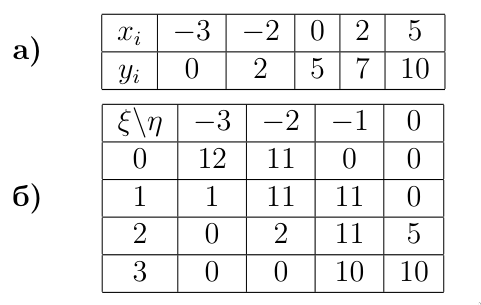
\includegraphics[width=5.5cm]{11.png}
	\\
}
Вважаю, що потрібно будувати регресію $y$ на $x$ та $\eta$ на $\xi$. Також за вказівкою лекторки знаходжу рівняння тільки лінійної регресії.

\paragraph{а) }

\begin{minted}{r}
> x_i_11 <- c(-3,-2,0,2,5)
> x_11 <- x_i_11
> y_11 <- c(0,2,5,7,10)

> a_11 <- data.frame(x_11, y_11)
> a_11$x2 = a_11$x_11^2
> a_11$y2 = a_11$y_11^2
> a_11$xy = a_11$x_11 * a_11$y_11

> a_11

  x_11 y_11 x2  y2 xy
1   -3    0  9   0  0
2   -2    2  4   4 -4
3    0    5  0  25  0
4    2    7  4  49 14
5    5   10 25 100 50
> sum(a_11$x2)

[1] 42
> sum(a_11$x_11)

[1] 2
> sum(a_11$xy)

[1] 60
> sum(a_11$y_11)

[1] 24
\end{minted}

\begin{figure}
	\centering
	\subcaptionbox{Очевидно, є лінійна залежність} {
	\includegraphics[width=.45\textwidth]{scatter_plot}
	}
	\subcaptionbox{Виглядає, як параболічна залежність, але даних замало, щоб сказати точно} {
	\includegraphics[width=.45\textwidth]{scatter_plot_2}
	}
	\caption{Графіки до 11 завдання}
\end{figure}

\paragraph{Складаємо систему, щоб знайти коефіцієнти рівняння $\bar y=ax+b$}

$$
\begin{cases}
	a \sum x_i^2 + b \sum x_i = \sum x_i y_i \\
	a \sum x_i + bn = \sum y_i
\end{cases}
\implies
\begin{cases}
	42*a + 2b = 60 \\
	2*a + b*5 = 24
\end{cases}
$$

\begin{align}
\Delta =
\begin{vmatrix}
	42 & 2 \\
	2 & 5
\end{vmatrix}
= 42*5-2*4 = 202
\\
\Delta_a =
\begin{vmatrix}
	60 & 2 \\
	24 & 5
\end{vmatrix}
= 60*5-2*24 = 252
\implies a = 252/202 = 1.(2475)
\\
\Delta_b =
\begin{vmatrix}
	42 & 60 \\
	2  & 24
\end{vmatrix}
= 42*24-2*60 = 888
\implies b = 888/202 = 4.(3960)
\end{align}

$$
\bar y = 1.(2475)x + 4.(3960)
$$

\paragraph{б)} Знаходимо рівняння лінійної регресії за формулою
% $$
% y = ax + b,
% a = \frac{r*\sigma_y}{\sigma_x},
% b = \bar y - a \bar x
% $$
$$
y - \bar y = r_{xy} * \frac{\sigma_y}{\sigma_x}(x-\bar x),\,
r_{xy} \text{(коефіцієнт кореляції)} = \frac{\overline{xy} - \bar x * \bar y}{\sigma_x\sigma_y}
$$

\subparagraph{Обчислення $\sigma_{\xi}, \bar \xi$}
\begin{minted}{r}
> xi_11 <- c(0,1,2,3)
> n_xi_11 <- c(23,23,18,20)
> xi_11_calc <- data.frame(xi_11, n_xi_11)
> xi_11_calc$xin = xi_11_calc$xi_11*xi_11_calc$n_xi_11
> xi_11_calc$xi2n = xi_11_calc$xi_11^2*xi_11_calc$n_xi_11
> xi_11_calc
  xi_11 n_xi_11 xin xi2n
1     0      23   0    0
2     1      23  23   23
3     2      18  36   72
4     3      20  60  180
> xi_avg <- sum(xi_11_calc$xin)/sum(n_xi_11)
> xi_avg
[1] 1.416667
# обчислення дисперсії та стандартного відхилення
> xi_11_n <- sum(n_xi_11)
> xi_11_n
[1] 84
> xi_11_var <- sum(xi_11_calc$xi2n)/xi_11_n - xi_avg^2
> xi_11_var
[1] 1.266865
> xi_11_sd <- sqrt(xi_11_var)
> xi_11_sd
[1] 1.125551
\end{minted}

\subparagraph{Те саме для $\eta$}

\begin{minted}{r}
> eta_11 <- c(-3,-2,-1,0)
> n_eta_11 <- c(13,24,32,15)
> eta_11_calc <- data.frame(eta_11, n_eta_11)
> eta_
eta_11       eta_11_calc  eta_dist     eta_p        eta_val
> eta_11_calc$etan <- eta_11_calc$eta_11*eta_11_calc$n_eta_11
> eta_11_calc$eta2n <- eta_11_calc$eta_11^2*eta_11_calc$n_eta_11
> eta_11_calc
  eta_11 n_eta_11 etan eta2n
1     -3       13  -39   117
2     -2       24  -48    96
3     -1       32  -32    32
4      0       15    0     0

> eta_11_n <- sum(n_eta_11)
> eta_11_n
[1] 84
> eta_avg <- sum(eta_11_calc$etan)/eta_11_n
> eta_avg
[1] -1.416667
> eta_11_sd <- sqrt(sum(eta_11_calc$eta2n)/eta_11_n - eta_avg^2)
> eta_11_sd
[1] 0.9537936

# обчислення середнього добутку xi*eta
> 0*12*(-3)+1*(-3)+0+11*(-2)+11*(-1)+2*2*(-2)+2*11*(-1)+0+3*10*(-1)
[1] -96
> -96/84
[1] -1.142857
\end{minted}

Нагадаю формулу коефіцієнта кореляції:
$
r_{{\xi}\eta} = \frac{\overline{{\xi}\eta} - \bar {\xi} * \bar \eta}{\sigma_{\xi}\sigma_\eta}
= ...
$

\begin{minted}{r}
> (-1.142857-xi_avg*eta_avg)/(xi_11_sd*eta_11_sd)
[1] 0.8048929
\end{minted}

$$
\eta - \bar \eta = r_{\xi\eta} * \frac{\sigma_\eta}{\sigma_x}(\xi-\bar \xi)
\implies
\eta - (-1.416667) = 0.8048929 * \frac{0.9537936}{1.125551}(\xi-1.416667)
$$

\Answer{
	\begin{enumerate}[a)]
		\item
$
\bar y = 1.(2475)x + 4.(3960)
$;

\item
$
% \eta + 1.416667 = 0.682067\xi-0.966262
\eta = 0.682067\xi-2.382929
$
	\end{enumerate}
}

\end{document}
